% lens_paper_v2.tex — MNRAS submission draft
% All edits from the editorial specification applied.
% Compiled with pdflatex.

\documentclass[fleqn,usenatbib]{mnras}

\usepackage{graphicx}
\usepackage{amsmath}
\usepackage{amssymb}
\usepackage{natbib}
\usepackage{hyperref}

% -----------------------------------------------------------------
\title[Background-Disjoint CV for Lens Classifiers]{Background-Disjoint Cross-Validation Reveals Hidden Failure Modes
in CNN Gravitational Lens Classifiers}

\author[M.\ Blumhardt]{Michael Blumhardt$^{1}$\\
$^{1}$Independent Researcher, Medford, OR, USA}

\date{Accepted XXX. Received XXX; in original form XXX}

\pubyear{2026}

\begin{document}
\label{firstpage}
\pagerange{\pageref{firstpage}--\pageref{lastpage}}
\maketitle

% =================================================================
% ABSTRACT
% =================================================================
\begin{abstract}
CNN-based gravitational lens finders are widely used in survey pipelines
and are commonly trained using simulated arc injections into real galaxy
images. Injection pipelines frequently generate multiple training samples
from the same background galaxy. Under standard image-level
cross-validation, images derived from a common background can appear in
both training and test folds, creating a leakage pathway through which
models can memorise background morphology and achieve optimistic
performance estimates.

Background-disjoint cross-validation (BDCV) eliminates this leakage
channel by assigning all images derived from a given background galaxy to
a single fold. Applied to a controlled dataset of 2,200 single-band
images (200 arc injections and 2,000 negatives) drawn from 217 unique
backgrounds, a convolutional neural network with approximately
$3.6\times10^5$ parameters yields FPR = 0.106 and AUC = 0.968 under
standard five-fold cross-validation. Background-disjoint evaluation
yields FPR = 0.145 and AUC = 0.917, revealing a 37 per cent increase in
false positives and a substantial reduction in recovery.

False positives are extremely concentrated across background galaxies.
The per-background false-positive distribution has Gini coefficient
$G = 0.879$, exceeding the maximum value obtained under 2,000
permutation replicates ($0.530$) by a margin of 0.35 and placing the
observed statistic completely outside the null support. Classical
photometric and morphological descriptors fail to distinguish catastrophic
from clean backgrounds, yet separation emerges in the learned
representation (embedding-space AUC = 0.947). Replication on an
independent parametric simulation of 150 S\'{e}rsic-profile backgrounds
yields standard CV FPR = 0.107 and BDCV FPR = 0.180.

Image-level cross-validation can therefore substantially underestimate
false-positive burden in injection-trained lens classifiers.
Background-disjoint cross-validation provides a simple evaluation
safeguard capable of revealing background-dependent shortcut behaviour.
\end{abstract}

\begin{keywords}
gravitational lensing: strong -- methods: statistical -- techniques:
image processing -- surveys
\end{keywords}

% =================================================================
% 1. INTRODUCTION
% =================================================================
\section{Introduction}
\label{sec:intro}

Gravitational strong lensing --- the formation of arcs and Einstein rings
when a massive foreground galaxy deflects light from a background source
--- provides powerful constraints on dark matter distributions,
cosmological parameters, and the mass structure of galaxies. Wide-field
photometric surveys are expected to yield tens of thousands of strong lens
candidates, far exceeding the capacity for visual inspection.

CNN-based lens finders are now widely used in survey pipelines
\citep{lanusse2018,petrillo2019,metcalf2019}. The standard training
approach injects simulated gravitational arcs into real galaxy images and
trains a binary classifier to distinguish injected images from unmodified
backgrounds.

Dataset bias and shortcut learning represent well-documented challenges
in machine-learning systems. Models frequently exploit correlations
present in training data rather than causal signals relevant to the
target task \citep{torralba2011,geirhos2020}. Similar concerns arise in
evaluation methodology, where standard validation protocols can mask
distribution shifts between training and deployment environments
\citep{recht2019}. Injection-trained lens classifiers possess a
structural property that creates an additional vulnerability: multiple
training samples may originate from the same background galaxy. Under
image-level cross-validation, this structure allows background morphology
to appear simultaneously in training and evaluation partitions,
potentially inflating apparent performance. To date, background identity
has not been used as a constraint in cross-validation protocols for
injection-trained lens classifiers.
Because injection pipelines are widely used to train automated lens
finders for current and upcoming surveys, evaluation protocols that
overlook this dependency structure may systematically underestimate the
operational false-positive burden.

This paper introduces background-disjoint cross-validation (BDCV) and
demonstrates that this methodological change reveals substantial
background-dependent failure modes invisible to standard evaluation.
Group-wise cross-validation has been applied in other domains, for
example patient-level splits in medical imaging. The contribution here
is the demonstration that background-identity constraints reveal a
systematic and quantifiable failure mode in injection-trained
astronomical classifiers.

% =================================================================
% 2. DATA AND METHODS
% =================================================================
\section{Data and Methods}
\label{sec:methods}

\subsection{Dataset}
\label{sec:dataset}

The dataset consists of 2,200 single-band $101\times101$-pixel images
drawn from 217 unique background galaxies: 200 positives (simulated arc
injections) and 2,000 negatives (unmodified backgrounds). Each background
contributes approximately 9--10 negatives and 0--1 positives. Images are
sky-subtracted single-band cutouts.

\subsection{Model}
\label{sec:model}

The classifier has approximately $3.6\times10^5$ parameters with a
128-dimensional penultimate embedding layer, using convolutional blocks
with batch normalisation and ReLU activations, global average pooling,
and a fully connected classification head.

\subsection{Background-disjoint cross-validation}
\label{sec:bdcv}

BDCV treats the background galaxy as the unit of assignment: all images
derived from a given background are assigned to the same fold. With
5-fold BDCV on 217 backgrounds, each test fold contains images from
approximately 43--44 unique backgrounds unseen during training.
Implementation requires only that images be grouped by background
identifier during fold construction (e.g.\ \textsc{GroupKFold} in
scikit-learn) and therefore imposes no additional computational cost
relative to standard cross-validation.

\subsection{Evaluation metrics}
\label{sec:metrics}

Performance is summarised by pooled false-positive rate (FPR),
true-positive rate (TPR), and mean fold-level AUC. The FPR target of
0.10 follows conventions used in the lens-finding literature; the
primary result, concentration of errors across backgrounds, is
independent of this threshold. A background is
classified as catastrophic when $\mathrm{FPR} = 1.0$ across all
negatives in that group. False-positive concentration is quantified using
the Gini coefficient computed over per-background FP counts, with
significance assessed by permutation test (2,000 replicates, seed = 42).
The permutation test preserves the total number of false positives while
randomly reallocating those errors across background groups, representing
the concentration expected under background-independent errors.

\begin{table}
\centering
\caption{Standard versus background-disjoint cross-validation. Same
dataset, architecture, hyperparameters, and seed; protocols differ only
in fold construction. Standard CV yields an apparently acceptable FPR
(0.106) but BDCV reveals a 37 per cent higher error rate and markedly
lower recovery.}
\label{tab:cv_comparison}
\begin{tabular}{lccc}
\hline
Evaluation protocol & AUC & TPR & FPR \\
\hline
Standard KFold       & 0.968 & 0.935 & 0.106 \\
Background-disjoint KFold & 0.917 & 0.781 & 0.145 \\
\hline
\end{tabular}
\end{table}

% =================================================================
% 3. RESULTS
% =================================================================
\section{Results}
\label{sec:results}

Background-disjoint evaluation reveals two striking empirical properties
of the classifier. First, standard
image-level cross-validation substantially underestimates the
false-positive burden when background identity is ignored during fold
construction. Second, false-positive errors are highly concentrated
across background galaxies rather than approximately uniform. Aggregating
fold-level predictions yields 289 false positives arising from only 32
of 217 background galaxies; 185 backgrounds produce no errors. The
false-positive distribution has Gini coefficient $G = 0.879$, far
outside a permutation null generated by random reallocation of errors
across backgrounds (null mean $0.463$, maximum $0.530$, 2,000
permutations). The observed statistic exceeds the entire null support by
a margin of $0.35$, indicating that the concentration cannot plausibly
arise from background-independent error allocation. Subsequent
subsections quantify the evaluation discrepancy, examine diagnostic
evidence for the failure mode structure, and present an independent
replication.

\subsection{Standard versus background-disjoint cross-validation}
\label{sec:cv_results}

Standard and background-disjoint 5-fold cross-validation results are
compared in Table~\ref{tab:cv_comparison}. Both protocols used the same
dataset, architecture, hyperparameters, and random seed, differing only
in fold construction. Performance differs substantially. Under ordinary
random 5-fold cross-validation the pooled FPR is 0.106, close to the
nominal target of 0.10, and the pooled TPR is 0.935. Under BDCV the
pooled FPR increases to 0.145 (+37 per cent), while TPR decreases to
0.781 ($-$15.4 percentage points). Mean validation AUC declines from
$0.968 \pm 0.028$ to $0.917 \pm 0.087$.

The change in performance is accompanied by a marked increase in error
heterogeneity. Standard CV identifies 9 catastrophic background groups
(those on which every negative is misclassified), whereas BDCV reveals
29 --- a 3.2-fold increase. Fold-to-fold FPR standard deviation
increases 2.3$\times$ and TPR standard deviation increases 4.1$\times$
under BDCV. Twenty backgrounds that appear completely clean under
standard evaluation produce $\mathrm{FPR} = 1.0$ when the model cannot
memorise them.

These results indicate that standard image-level cross-validation can
produce optimistic performance estimates when background realisations
appear in both training and test partitions. The injected-data
construction is critical: because arc injections are generated
independently of background morphology, no astrophysically legitimate
correlation exists between background structure and lens presence in this
dataset; any predictive dependence on background morphology therefore
reflects shortcut use within the learned representation rather than
genuine lensing signal.

\subsection{False-positive concentration across background galaxies}
\label{sec:fp_concentration}

Under BDCV the pooled FPR is 0.145, exceeding the target of 0.10. This
excess is not distributed uniformly. Aggregating from the five
fold-level prediction files yields 289 false positives across 217
backgrounds (mean = 1.33 per group). Of 217 backgrounds, 185 produce no
false positives. The remaining 32 backgrounds produce at least one false
positive, while 29 backgrounds are catastrophic
($\mathrm{FPR} = 1.0$). Each catastrophic background contributes
approximately 9--10 negatives; FPR = 1.0 therefore represents consistent
misclassification of all images from that background rather than a
single-image artifact. Error concentration is itself highly skewed: 22
backgrounds (10.1 per cent) account for 80 per cent of all errors
(Fig.~\ref{fig:fp_concentration}). The Gini coefficient is $G = 0.879$;
a permutation test yields $p < 5\times10^{-4}$ (2,000 permutations).
The observed statistic exceeds the maximum value obtained in 2{,}000
permutations by $0.35$, placing the observed concentration far outside
the range expected under background-independent error allocation.

\begin{figure}
\centering
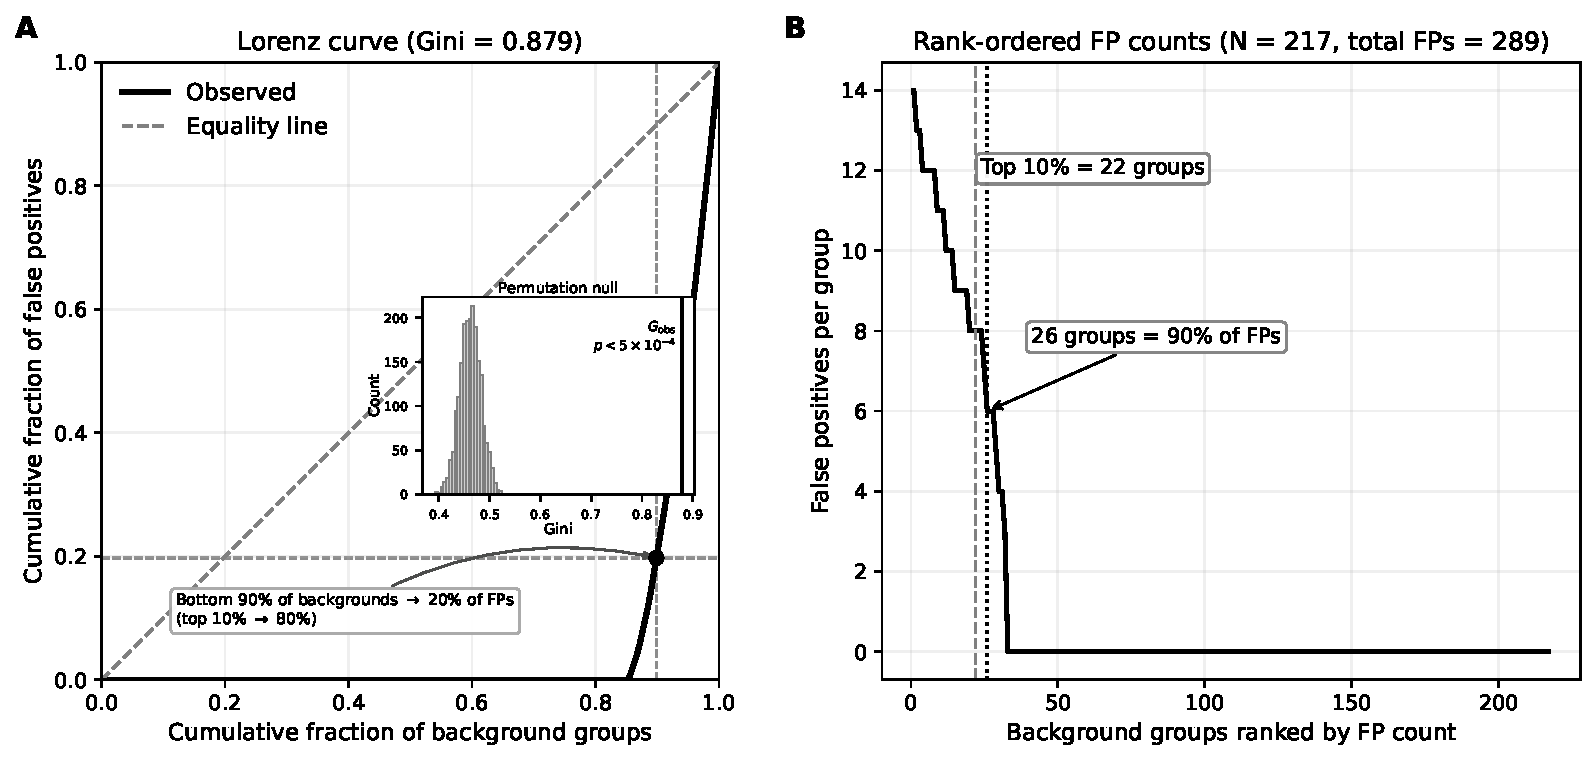
\includegraphics[width=\columnwidth]{figures/fp_concentration_twopanel.pdf}
\caption{Left: false positives per background group, ranked in
decreasing order. Right: Lorenz curve across all 217 groups. Gini =
0.879; 22 groups (10.1 per cent) account for 80 per cent of all 289
errors. Permutation $p < 5\times10^{-4}$.}
\label{fig:fp_concentration}
\end{figure}

\begin{figure}
\centering
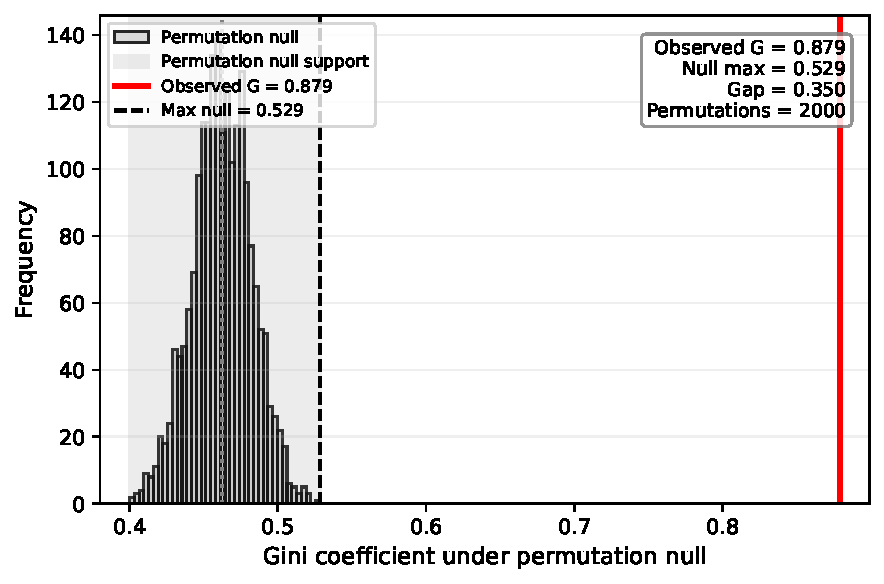
\includegraphics[width=\columnwidth]{figures/gini_permutation_null_histogram.pdf}
\caption{Permutation null distribution of the false-positive Gini
coefficient (2,000 replicates; FP counts randomly reallocated across 217
background groups preserving the observed total of 289). The null
distribution (grey histogram) is compact and approximately symmetric
(mean = 0.463, SD = 0.020, max = 0.530). The observed Gini coefficient
$G = 0.879$ (red vertical line) lies 0.35 above the null maximum,
exceeding all 2,000 replicates ($p < 5\times10^{-4}$). The empty gap
between the null support and the observed value indicates that the
concentration cannot plausibly arise from random error allocation across
backgrounds.}
\label{fig:gini_null}
\end{figure}

Additional perturbation tests produced qualitatively consistent behaviour
but introduced masking artefacts that complicate interpretation; the
primary inference therefore relies on the concentration statistic and
representation analysis.

Visual inspection of the six highest-error catastrophic groups confirms
that the operative confounders are large-scale morphological features of
the background galaxies themselves (Fig.~\ref{fig:catastrophic_examples}).
Confounders include tidal streams, off-axis compact source
configurations, and absorbing features with arc-like curvature. The
injected arc signal is not visible at the display stretch used,
confirming that the classifier response is dominated by pre-existing
background structure.

\begin{figure}
\centering
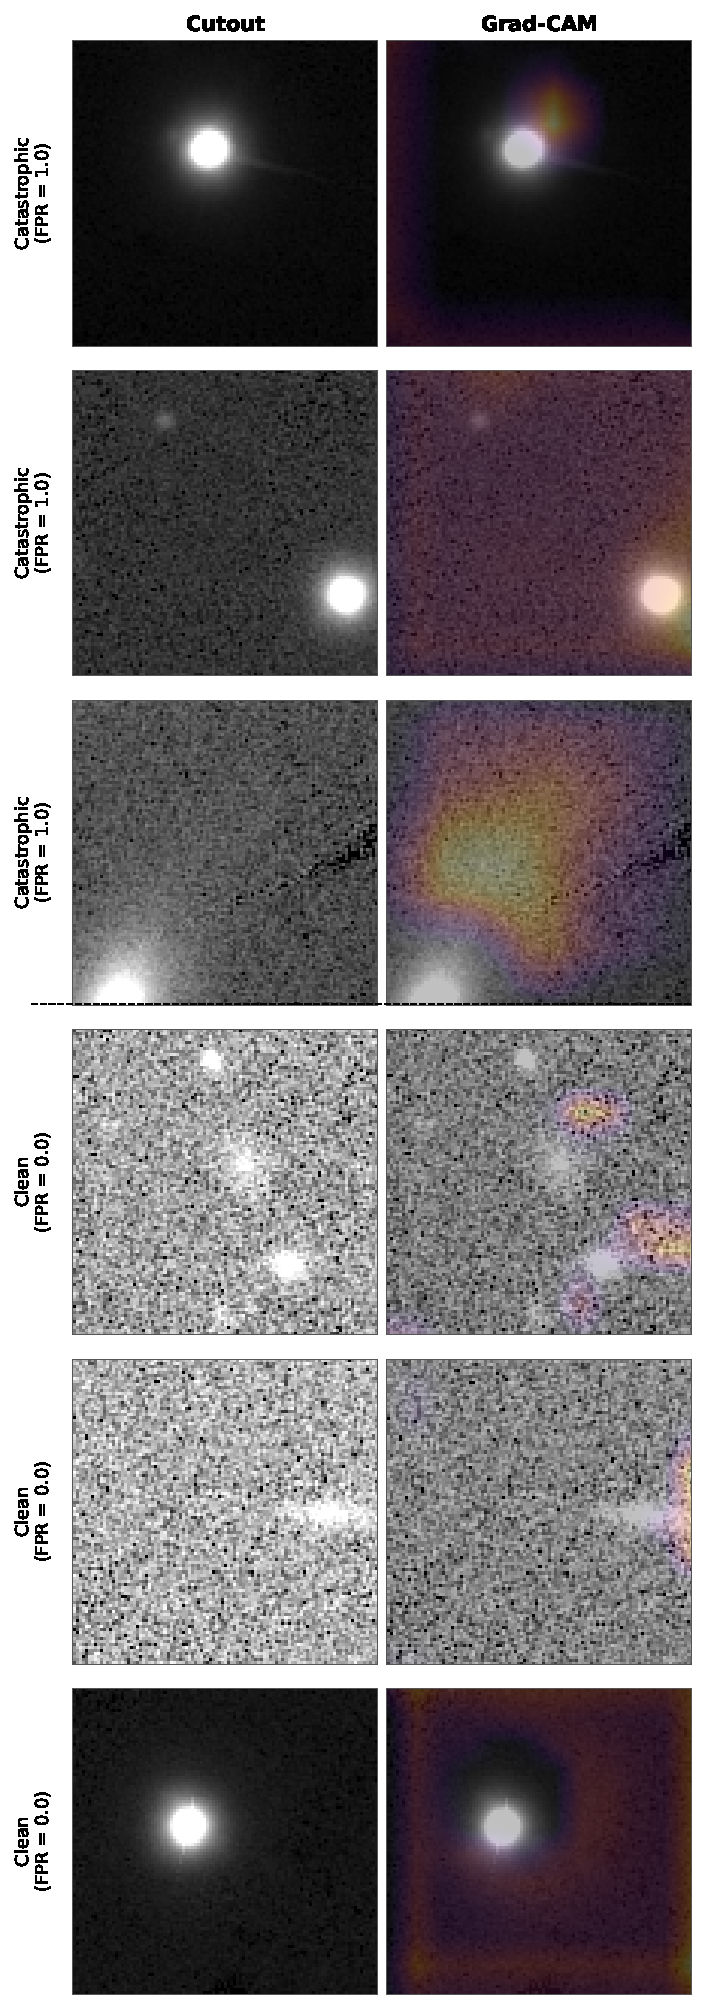
\includegraphics[width=\columnwidth,height=0.85\textheight,keepaspectratio]{figures/gradcam_catastrophic_vs_clean.pdf}
\caption{Catastrophic background groups. Each row shows (left) the
background galaxy, (centre) a false-positive negative, and (right) a
simulated arc injection from the same background at identical display
stretch. The arc signal is not visible; classifier activation is driven
by pre-existing background morphology.}
\label{fig:catastrophic_examples}
\end{figure}

Kolmogorov--Smirnov tests on sky coordinates of catastrophic versus
clean groups yield $p = 0.81$ (RA) and $p = 0.68$ (Dec), ruling out
spatial clustering or field-level artefacts
(Fig.~\ref{fig:sky_distribution}).

\begin{figure}
\centering
\includegraphics[width=\columnwidth]{../artifacts/groupkfold/gkf_unweighted_seed0/catastrophic_groups_spatial.png}
\caption{Sky distribution of catastrophic (red crosses) and clean (blue
circles) background groups. KS tests: $p = 0.81$ (RA), $p = 0.68$
(Dec). No spatial clustering.}
\label{fig:sky_distribution}
\end{figure}

Across three rounds of progressively detailed morphological analysis, no
tested interpretable morphology statistic distinguished catastrophic from
clean groups. Spearman correlations between CNN logit and scalar metrics
(peak surface brightness, total flux, half-light radius, concentration
index) across all 2,000 negatives are all $|\rho| < 0.012$, $p > 0.6$
(Fig.~\ref{fig:logit_brightness}). Peak surface brightness, the
classical predictor most likely to correlate with both background
morphology and classifier response, shows Spearman $|\rho| < 0.02$
($p > 0.6$), ruling out brightness as the operative confounder. Azimuthally averaged radial profiles
show no significant difference at any of 35 radius bins. A panel of 15
non-radial 2-D features --- Sobel edge strength and orientation entropy,
asymmetry residuals, ellipticity, arcness, and PCA components --- yields
zero of 30 feature--aggregation pairs at $p < 0.05$, with all effect
sizes $|r| < 0.2$. The operative feature therefore likely resides in a
distributed representation that is not preserved by the summary
statistics considered here.

\begin{figure}
\centering
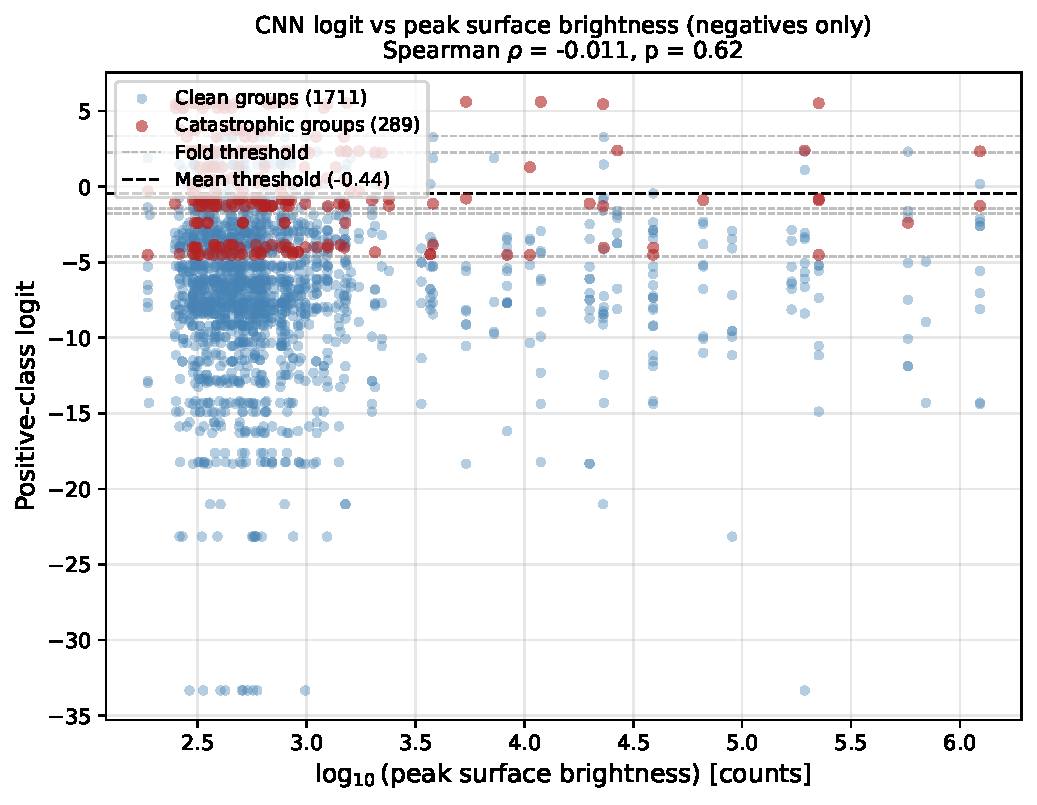
\includegraphics[width=\columnwidth]{figures/logit_vs_peak_surface_brightness.pdf}
\caption{CNN logit vs.\ $\log_{10}$ peak surface brightness for all
2,000 negatives. Catastrophic (red) and clean (blue) images overlap
across the full brightness range. Spearman $|\rho| < 0.02$, $p > 0.6$
for all scalar metrics.}
\label{fig:logit_brightness}
\end{figure}

% --- Section 3.3 ---
\subsection{Embedding-space separation and Grad-CAM attribution}
\label{sec:embedding_gradcam}

The following analyses investigate the representation-level structure of
the failure mode and are presented as mechanistic diagnostic evidence
rather than as the primary statistical result.

Catastrophic and clean background groups were not distinguishable using
the classical photometric and morphology descriptors tested above. In
contrast, the same groups are strongly separable in the model's learned
representation. Using the 128-dimensional penultimate embedding extracted
from out-of-fold models, a leave-one-out logistic regression classifier
distinguished catastrophic ($\mathrm{FPR} = 1.0$) from clean
($\mathrm{FPR} = 0.0$) background groups with AUC = 0.947 (permutation
$p < 0.005$). Catastrophic groups do not form a visually distinct
cluster (silhouette = 0.036); nearest-neighbour purity is modest ($k=5$:
0.64; $k=10$: 0.56). Discriminative signal is carried by minor PCA
components (PC3, $p = 0.001$; PC5, $p = 3.6\times10^{-5}$) rather than
dominant variance directions. When coloured by mean classifier logit,
the embedding reveals a continuous mapping from background type to
prediction score, with catastrophic groups occupying regions of feature
space associated with systematically higher positive-class logits
(Fig.~\ref{fig:embedding_pca}).

This result establishes that the failure mode is encoded in the model's
internal representation even though it is not captured by the tested
classical descriptors. Within the feature families evaluated here, no
standard astronomical summary statistic reproduces this separation.

\begin{figure}
\centering
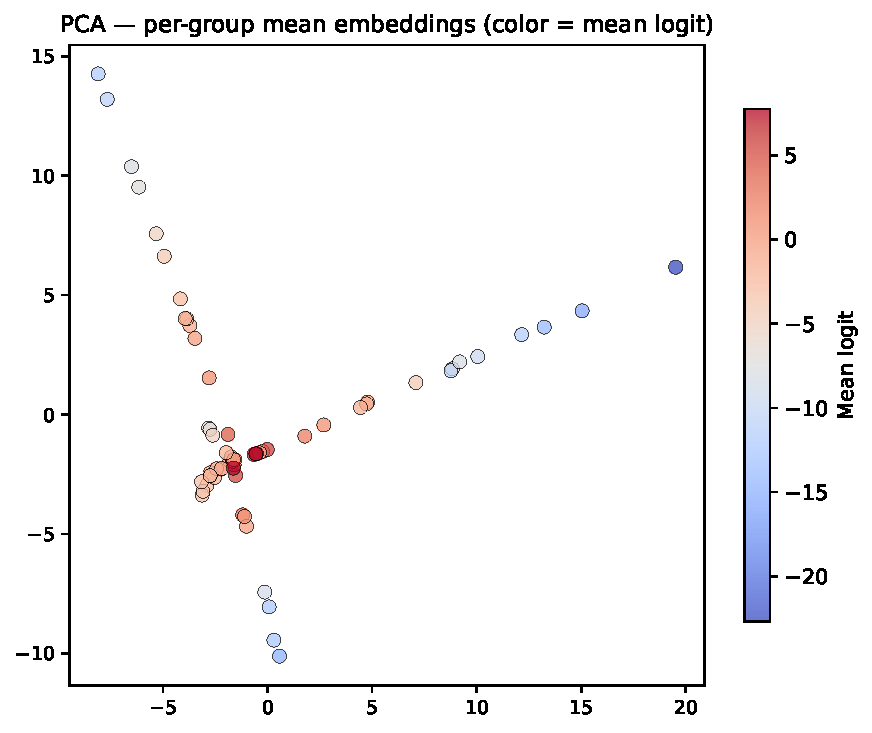
\includegraphics[width=\columnwidth]{figures/embedding_pca_per_group_logit.pdf}
\caption{PCA of per-group mean embeddings coloured by mean
positive-class logit. Catastrophic groups (warm colours, high logit)
concentrate centrally; clean groups (cool colours) scatter to the
periphery. LOO logistic AUC = 0.947 ($p < 0.005$) in the full
128-dimensional space.}
\label{fig:embedding_pca}
\end{figure}

To localise the spatial basis of this learned failure mode,
Grad-CAM\footnote{Grad-CAM attribution maps were computed from models
retrained under the same background-disjoint fold structure because
fold-level checkpoints from the canonical experiment were not retained.
Attribution analyses therefore characterise typical model behaviour under
the protocol rather than the exact parameter realisations used in the
primary evaluation.} attribution maps \citep{selvaraju2017} were
computed for catastrophic and clean background groups. Qualitative
examples are shown in Fig.~\ref{fig:gradcam_examples}. Catastrophic
backgrounds exhibit stronger and more spatially coherent positive-class
attribution on off-centre galaxy structure, including curved outer
features and surrounding halo emission, whereas clean backgrounds
typically show weaker or less coherent activation.

\begin{figure}
\centering
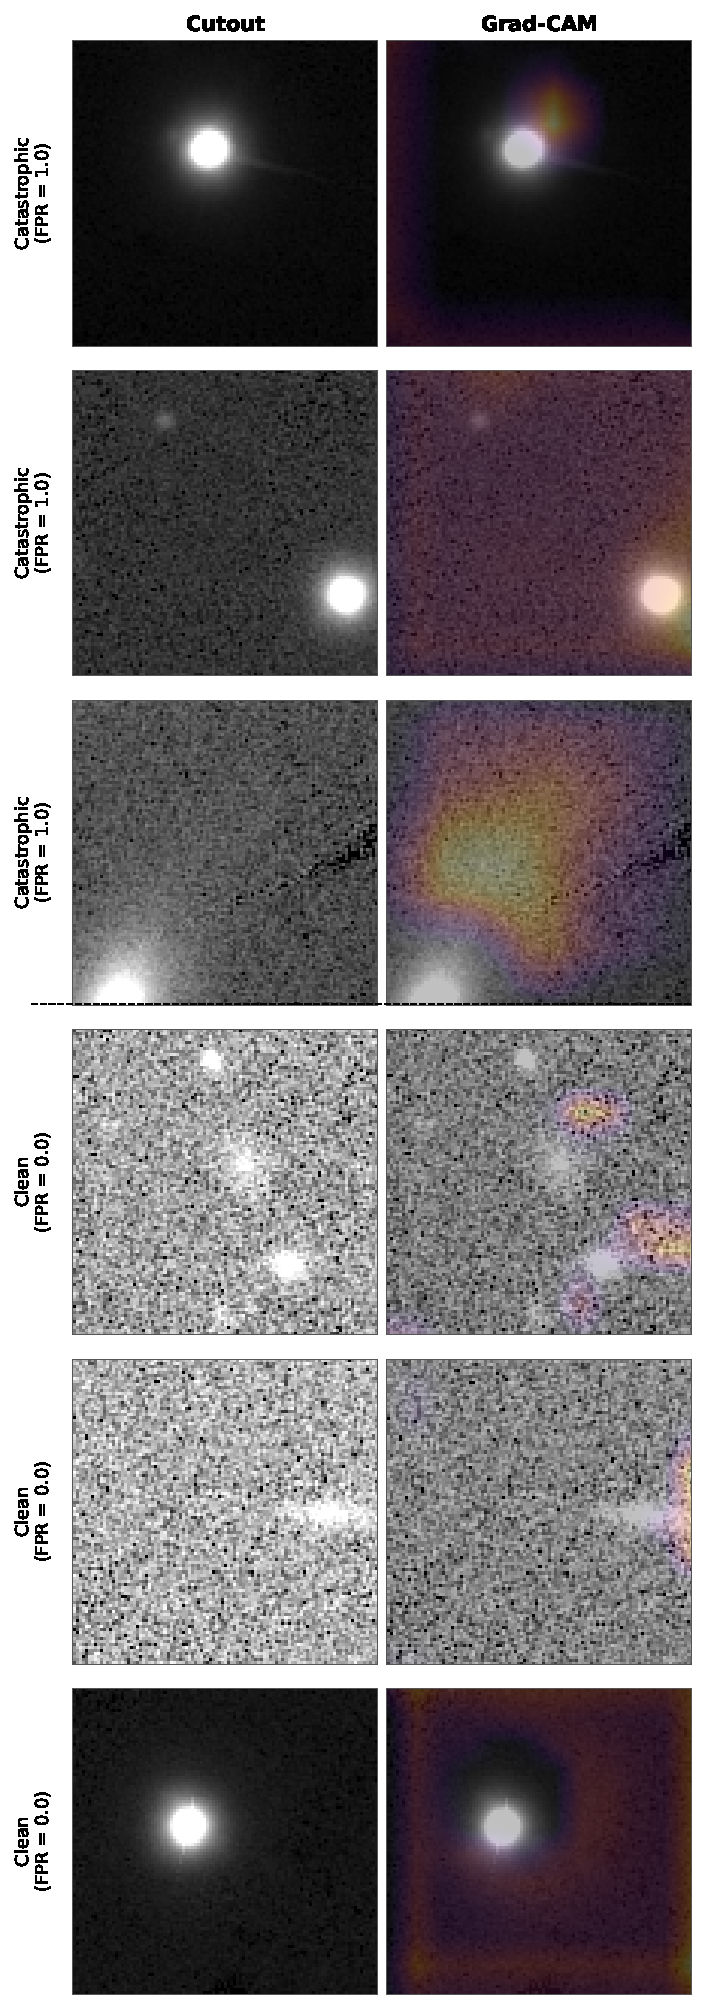
\includegraphics[width=\columnwidth,height=0.85\textheight,keepaspectratio]{figures/gradcam_catastrophic_vs_clean.pdf}
\caption{Grad-CAM attribution for catastrophic (top 3 rows,
$\mathrm{FPR} = 1.0$) and clean (bottom 3 rows, $\mathrm{FPR} = 0.0$)
background groups. Left: normalised cutouts; right: Grad-CAM overlays.
Catastrophic groups show stronger, more coherent attribution on outer
halo structure consistent with a morphology-driven shortcut in which
curved halo structure activates the positive-class pathway.}
\label{fig:gradcam_examples}
\end{figure}

Quantitative attribution summaries were computed for all 29 catastrophic
groups (289 images) and 32 matched clean groups (313 images). Attribution
concentration was not stable across two independent retraining runs
($p = 2.3\times10^{-6}$ in one run, $p = 0.068$ in another) and is not
treated as a primary inferential result. Two attribution patterns were
robust. Peak outer attribution is consistently higher for catastrophic
groups ($0.454 \pm 0.426$ vs $0.341 \pm 0.397$, $p = 2.2\times10^{-4}$),
confirming activation in the 10--35 pixel annulus where lensing arcs
appear in training. Attribution asymmetry is consistently lower for
catastrophic groups (median 3.5 vs 10.0, $p < 10^{-11}$), indicating
more spatially balanced activation (Fig.~\ref{fig:gradcam_boxplot}).

\begin{figure}
\centering
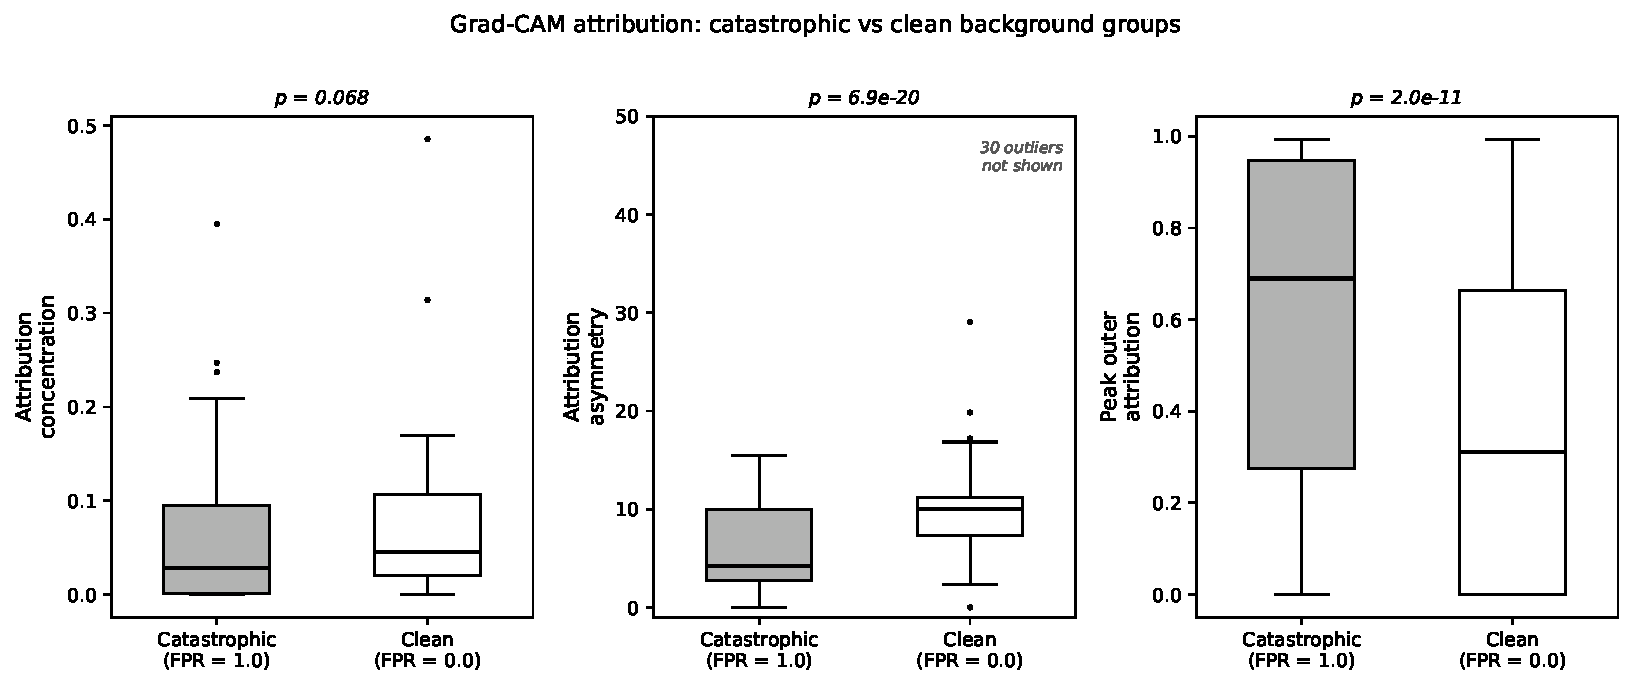
\includegraphics[width=\columnwidth]{figures/gradcam_summary_boxplot.pdf}
\caption{Quantitative Grad-CAM summary. Left: attribution concentration
(not stable across retraining runs; descriptive only). Centre:
attribution asymmetry (lower for catastrophic --- more spatially
balanced). Right: peak outer attribution (higher for catastrophic ---
outer halo activation). Asymmetry and peak outer attribution are stable
across independent retraining runs and are treated as primary results.}
\label{fig:gradcam_boxplot}
\end{figure}

The embedding and attribution results are complementary. The embedding
analysis shows that catastrophic and clean backgrounds are strongly
separable in the learned representation despite being indistinguishable
under tested classical morphology summaries. The Grad-CAM analysis shows
that this representation is expressed spatially through increased
reliance on off-centre background structure at arc-relevant radii.
Together these analyses are consistent with a background-dependent
failure mode in which the CNN has learned a representation that maps
specific galaxies to regions of feature space associated with elevated
lens logits, expressed through activation on distributed outer-galaxy
structure rather than any simple brightness or compactness cue.

% --- Section 3.4: Independent replication ---
\subsection{Independent replication}
\label{sec:replication}

To test whether the observed error concentration is specific to the PS1
empirical backgrounds used in the primary experiment, the analysis was
repeated on an independent parametric simulation generated with the
\textsc{lenstronomy} pipeline \citep{birrer2018}. Replication on 150
S\'{e}rsic-profile backgrounds yields standard CV FPR = 0.107 and BDCV
FPR = 0.180. The standard-CV vs.\ BDCV gap and elevated fold-level
variance under BDCV are consistent with the primary PS1 result,
supporting robustness across simulation settings. BDCV identifies 24
catastrophic groups ($\mathrm{FPR} = 1.0$) and FP Gini = 0.819
(Fig.~\ref{fig:replication}).

\begin{figure}
\centering
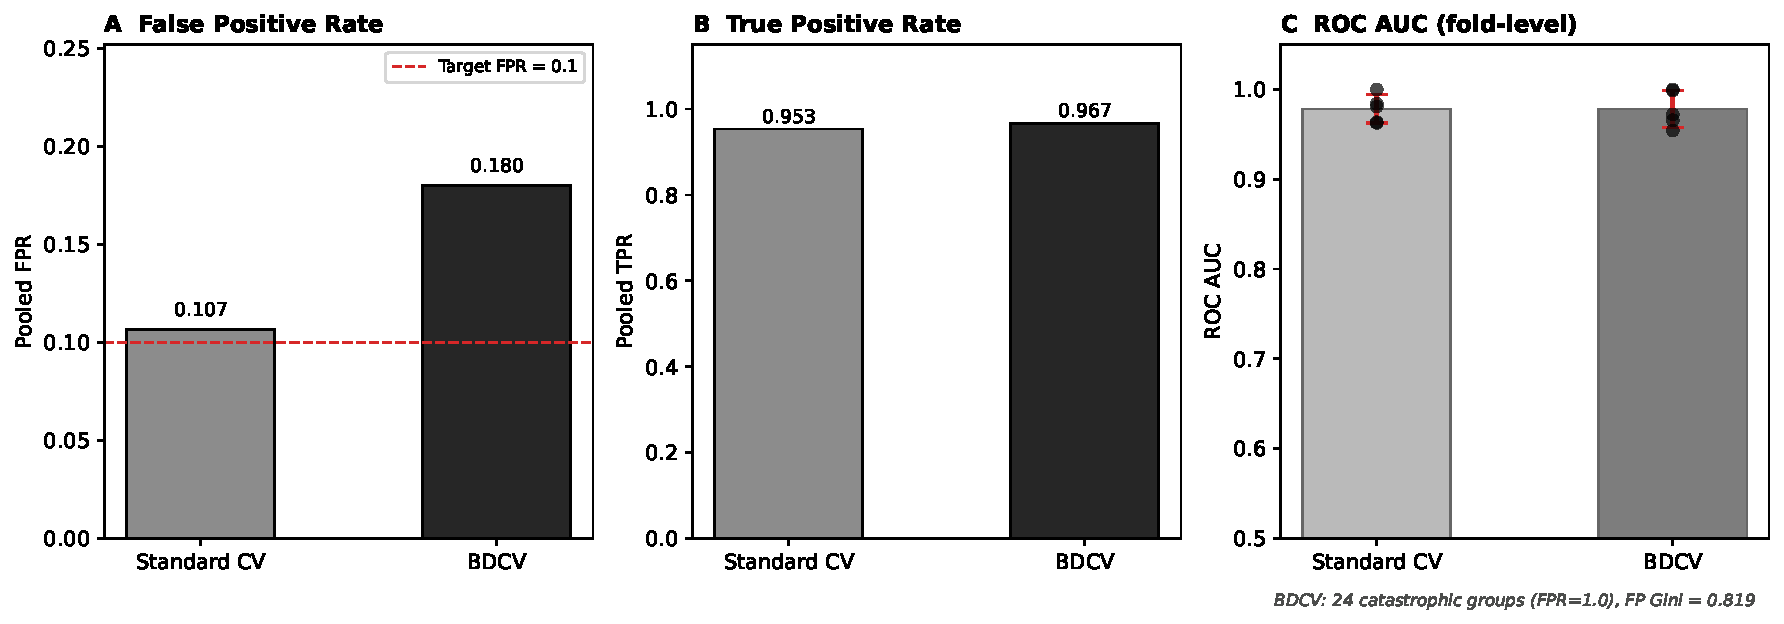
\includegraphics[width=\columnwidth]{figures/external_replication_bdcv_vs_standard.pdf}
\caption{Replication on an independent parametric simulation (150
S\'{e}rsic-profile backgrounds, \textsc{lenstronomy} pipeline). Panel A:
pooled FPR under standard CV (0.107) and BDCV (0.180); dashed red line
indicates the FPR target of 0.10. Panel B: pooled TPR. Panel C:
fold-level AUC with individual fold values shown. The standard-CV vs.\
BDCV gap and elevated fold-level variance under BDCV are consistent with
the primary PS1 result, supporting robustness across simulation settings.
BDCV: 24 catastrophic groups ($\mathrm{FPR} = 1.0$), FP Gini = 0.819.}
\label{fig:replication}
\end{figure}

Taken together, the concentration result, the spatial null result, the
morphological null results, the Grad-CAM attribution analysis, and the
embedding geometry provide a coherent account of the observed failure
mode. The CNN has learned a
background-dependent feature representation encoded in minor principal
components of the 128-dimensional embedding space that are not captured
by the standard photometric and morphology descriptors evaluated here.
This representation drives classification decisions that are invisible
to background-unaware evaluation: the same backgrounds that produce
$\mathrm{FPR} = 1.0$ under BDCV appear indistinguishable from safe
backgrounds by every classical morphology metric, yet are strongly
separated in the CNN's own internal representation. Background-disjoint
cross-validation is a low-cost evaluation safeguard that can reveal
background-dependent failure modes hidden by image-level cross-validation.

% =================================================================
% 4. DISCUSSION
% =================================================================
\section{Discussion}
\label{sec:discussion}

\subsection{Mechanism of the shortcut}
\label{sec:mechanism}

The injected-data design is critical for causal interpretation. Because
simulated lens signals are assigned independently of background identity,
no astrophysically legitimate correlation exists between background
morphology and the presence of a lens in this dataset. Predictive
dependence on background structure must therefore arise from shortcut use
rather than from any true lensing signal. This pattern is characteristic
of shortcut learning in deep convolutional models \citep{geirhos2020},
where predictive signals arise from combinations of weak cues distributed
across many spatial filters rather than from a single physically
interpretable feature. The permutation null tests whether the observed
error concentration exceeds what would arise if false positives were
allocated independently of background identity; within-group error
correlation is the phenomenon under investigation, not a confound of the
null model.

If catastrophic backgrounds simply represented intrinsically difficult
morphologies, performance would be expected to degrade gradually across
backgrounds under both evaluation protocols. Instead, the failure is
discrete and background-specific: several backgrounds produce
$\mathrm{FPR} = 1.0$ under BDCV while remaining error-free under
standard cross-validation, whereas most backgrounds produce no errors
under either protocol. This pattern is difficult to reconcile with a
continuous difficulty gradient and is consistent with
background-specific memorisation.

In real astronomical data, background morphology correlates with lensing
probability through the host galaxy population. The present result is
specific to injection-trained datasets where that correlation is absent
by construction.

\subsection{Implications for injection-trained lens finders}
\label{sec:implications}

Standard cross-validation suggests the model satisfies the target
false-positive rate, whereas background-disjoint evaluation reveals a 37
per cent higher FPR and substantially lower recovery, demonstrating that
image-level splitting conceals background leakage. Because many
lens-finding pipelines are trained using simulated arc injections into
real galaxies, similar correlations between training and test samples can
arise whenever evaluation protocols ignore background identity.
Background-disjoint cross-validation provides a simple and
computationally inexpensive evaluation safeguard that can reveal such
background-dependent failure modes before models are deployed in survey
pipelines. The aggregate FPR increase from 0.106 to 0.145 does not fully
convey the practical consequence of the failure mode. Standard evaluation
identifies 9 catastrophic backgrounds; BDCV reveals 29. A classifier
deployed after standard evaluation will systematically misclassify every
image from 20 background galaxy types that its own evaluation protocol
identified as safe.

\subsection{Limitations}
\label{sec:limitations}

Several limitations constrain the scope of the results. The analysis is
restricted to a single-band, injection-trained setting, and multiband
information may reduce reliance on morphology-based shortcuts by
providing colour contrast between foreground lenses and background
sources. The experiment is conducted on a controlled dataset comprising 217
unique background galaxies and one CNN architecture; results should be
interpreted as a controlled diagnostic demonstration. The sample is
adequate for the concentration analysis, where the relevant unit is the
background group rather than the individual image, but modest as a
training corpus.
The embedding-space separation result uses the same model whose failure
is being characterised. The analysis demonstrates that the failure mode
is encoded within the learned representation but cannot independently
establish which specific property of background morphology is causally
responsible. The observed Gini coefficient exceeds the permutation null
maximum by 0.35, a margin that cannot be attributed to small-sample
variance. Whether
attention-based or transformer architectures are more
or less susceptible to this failure mode is unknown; the concern is likely
general to any injection-trained model, but calibration on other
architectures remains warranted. Mitigation strategies such as
adversarial invariance, targeted augmentation, or hard-negative
retraining are not benchmarked here. The contribution is methodological
and diagnostic: to show that background-disjoint evaluation can reveal a
background-dependent failure mode that standard image-level validation
may miss.

% =================================================================
% 5. CONCLUSIONS
% =================================================================
\section{Conclusions}
\label{sec:conclusions}

Background-disjoint cross-validation reveals substantial failure modes in
CNN lens classifiers invisible to standard evaluation. The principal
findings are:

\begin{enumerate}
\item Standard CV achieves FPR = 0.106 and AUC = 0.968, apparently
meeting the target. BDCV reveals FPR = 0.145 (+37 per cent) and AUC =
0.917.

\item Error distribution is extremely concentrated: Gini = 0.879,
permutation $p < 5\times10^{-4}$; the observed statistic exceeds the
permutation null maximum by 0.35; 22 of 217 backgrounds account for 80
per cent of all 289 errors. Standard CV identifies 9 catastrophic
backgrounds; BDCV reveals 29.

\item Spatial KS tests ($p = 0.81$, 0.68) rule out field-level
artefacts.

\item All tested morphological metrics --- scalar, radial, and 15
non-radial 2-D features --- fail to distinguish catastrophic from clean
backgrounds.

\item A linear classifier in the CNN's 128-dimensional penultimate
embedding separates catastrophic from clean groups with LOO AUC = 0.947
($p < 0.005$).

\item Background-disjoint evaluation provides a simple, low-cost
safeguard that can reveal background-dependent failure modes before
deployment.

\item Independent replication on 150 S\'{e}rsic-profile backgrounds
(\textsc{lenstronomy} pipeline) yields standard CV FPR = 0.107 and BDCV
FPR = 0.180, with 24 catastrophic groups and FP Gini = 0.819, confirming
that the result is not specific to the PS1 empirical backgrounds.
\end{enumerate}

Background-disjoint cross-validation therefore provides a simple
evaluation safeguard capable of revealing background-dependent shortcut
behaviour that remains hidden under conventional image-level validation.

% =================================================================
% ACKNOWLEDGEMENTS
% =================================================================
\section*{Acknowledgements}

This research made use of \textsc{lenstronomy} \citep{birrer2018},
\textsc{astropy} \citep{astropy2013}, \textsc{scikit-learn}, and
\textsc{PyTorch}.

% =================================================================
% REFERENCES
% =================================================================
\begin{thebibliography}{99}

\bibitem[\protect\citeauthoryear{Astropy Collaboration}{2013}]{astropy2013}
Astropy Collaboration, 2013, A\&A, 558, A33

\bibitem[\protect\citeauthoryear{Birrer \& Amara}{2018}]{birrer2018}
Birrer S., Amara A., 2018, Phys.\ Dark Univ., 22, 189

\bibitem[\protect\citeauthoryear{Geirhos et~al.}{2020}]{geirhos2020}
Geirhos R., Jacobsen J.-H., Michaelis C., Zeiler M., Brendel W.,
Bethge M., Wichmann F.~A., 2020, Nat.\ Mach.\ Intell., 2, 665

\bibitem[\protect\citeauthoryear{Jacobs et~al.}{2017}]{jacobs2017}
Jacobs C., Glazebrook K., Collett T., More A., McCarthy C., 2017, ApJ,
841, 6

\bibitem[\protect\citeauthoryear{Jacobs et~al.}{2019}]{jacobs2019}
Jacobs C., Collett T., Glazebrook K., et~al., 2019, MNRAS, 484, 5330

\bibitem[\protect\citeauthoryear{Lanusse et~al.}{2018}]{lanusse2018}
Lanusse F., Ma Q., Li N., et~al., 2018, MNRAS, 473, 3895

\bibitem[\protect\citeauthoryear{Marshall et~al.}{2016}]{marshall2016}
Marshall P.~J., et~al., 2016, MNRAS, 455, 1171

\bibitem[\protect\citeauthoryear{Metcalf et~al.}{2019}]{metcalf2019}
Metcalf R.~B., Meneghetti M., Avestruz C., et~al., 2019, A\&A, 625,
A119

\bibitem[\protect\citeauthoryear{Petrillo et~al.}{2019}]{petrillo2019}
Petrillo C.~E., Tortora C., Vernardos G., et~al., 2019, MNRAS, 482,
807

\bibitem[\protect\citeauthoryear{Recht et~al.}{2019}]{recht2019}
Recht B., Roelofs R., Schmidt L., Shankar V., 2019, in Proc.\ ICML,
PMLR 97, pp 5389--5400

\bibitem[\protect\citeauthoryear{Selvaraju et~al.}{2017}]{selvaraju2017}
Selvaraju R.~R., Cogswell M., Das A., Vedantam R., Parikh D., Batra D.,
2017, in Proc.\ ICCV, pp 618--626

\bibitem[\protect\citeauthoryear{Torralba \& Efros}{2011}]{torralba2011}
Torralba A., Efros A.~A., 2011, in Proc.\ CVPR, pp 1521--1530

\end{thebibliography}

\label{lastpage}
\end{document}
